\chapter{Shock Waves}
\label{cha:shock-waves}\label{sec:shock-waves}
\index{fluid mechanics!shock waves}
\index{shocks}

\section{Non-relativistic Shocks}
\label{sec:non-relat-shocks}
\index{fluid mechanics!non-relativistic shock waves}
\index{shocks!non-relativistic}

Discontinuities signal a failure of fluid mechanics as we have
formulated it.   Fluid mechanics assumes that the material is
continuous so quantities cannot change discontinuously.  In practice
viscosity and thermal conduction save the day, so although the wave
may get really steep, a discontinuity doesn't actually form.  To
understand the structure of a shock, one needs to include viscosity,
but one can understand the behaviour of shocks without including
viscosity as we shall see.

Let's stand in the frame of the shock.  The fluid approaches the shock
supersonically on the left side and exits subsonically on the right
side.   Let $P_1, \rho_1$ and $v_1$ denote the physical quantities on
the left-hand side (the pre-shock fluid) and $P_2, \rho_2$ and $v_2$
in the post-shock fluid. 

First we have
\begin{equation}
\rho_1 v_1 = \rho_2 v_2 = j.
\label{eq:701}
\end{equation}
What goes into the shock must come out of the shock.  If you remember
the energy flux for an ideal fluid is
\begin{equation}
{\bf q} = \left [ \frac{1}{2} V^2 + w \right ] \rho {\bf V} .
\label{eq:702}
\end{equation}
This flux must be the same on each side (unless the shock is
radiative) so we have
\begin{equation}
\left ( \frac{1}{2} v_1^2 + w_1  \right ) \rho_1 v_1 = 
\left ( \frac{1}{2} v_2^2 + w_2  \right ) \rho_2 v_2 .
\label{eq:703}
\end{equation}
Because of conservation of mass we can simplify this to
\begin{equation}
 \frac{1}{2} v_1^2 + w_1 = \frac{1}{2} v_2^2 + w_2.
\label{eq:704}
\end{equation}
This states that the sum of the kinetic and internal energy per unit
mass is conserved across the shock.   Third we have to conserve the
momentum flux
\begin{equation}
P_1 + \rho_1 v_1^2 = P_2 + \rho_2 v_2^2
\label{eq:705}
\end{equation}
We can use the defintion of the enthalpy to eliminate it from the
equations
\begin{equation}
w = \epsilon + \frac{P}{\rho} = \frac{\gamma}{\gamma-1} \frac{P}{\rho} = 
 \frac{\gamma}{\gamma-1} k_B T.
\end{equation}
Let's define the Mach number of the incoming flow as $M_1=v_1/c_s$ and
rewrite Eq.~\ref{eq:705} as
\begin{equation}
\frac{P_2}{P_1} = 1 + \frac{\rho_1}{P_1} v_1^2 - \frac{\rho_2}{P_1}
v_2^2 = 1 + \gamma M_1^2 \left ( 1 -  \frac{\rho_1}{\rho_2} \right ).
\label{eq:837}
\end{equation}
We can also rewrite Eq.~\ref{eq:704} to yield
\begin{equation}
\frac{P_2}{P_1} = \frac{\rho_2}{\rho_1} + \frac{1}{2} M_1^2 \left
  (\gamma-1\right ) \left( \frac{\rho_2}{\rho_1} -
  \frac{\rho_1}{\rho_2} \right )
\label{eq:842}
\end{equation}
and we can equate these two expressions to solve for $\rho_2/\rho_1$.
From inspection we see that one solution is $\rho_2=\rho_1$, which
means that there is not discontinuity.   The other solution yields
\begin{eqnarray}
\frac{\rho_2}{\rho_1} = \frac{v_1}{v_2} &=& \frac{(\gamma+1) + (\gamma+1)
( M_1^2 - 1 )}{(\gamma+1)+(\gamma-1) (M_1^2-1)} = \frac{(\gamma+1)
  M_1^2}{2 + M_1^2 (\gamma-1)} \label{eq:679}\\
\frac{P_2}{P_1} &=&  \frac{(\gamma+1) + 2\gamma (M_1^2 -
  1)}{(\gamma+1)} = \frac{1-\gamma + 2 M_1^2 \gamma }{(\gamma+1)}, \\
\frac{T_2}{T_1} &=& \frac{(1-\gamma+2 M_1^2 \gamma) [2 + M_1^2
  (\gamma-1)]}{(\gamma+1)^2 M_1^2} \\
M_2^2 &=& \frac{(\gamma+1)+(\gamma-1) (M_1^2-1)}{(\gamma+1) + 2\gamma (M_1^2 -
  1)} = \frac{2+M_1^2(\gamma-1) }{1 - \gamma + 2  M_1^2\gamma}
\label{eq:706}
\end{eqnarray}
where intermediate expressions are given to show that if $M_1>1$, then
$\rho_2>\rho_1$, $P_2>P_1$ and $M_2<1$.
The fluid enters the shock supersonically and leaves the
shock subsonically.  The post-shock fluid has higher pressure and
density.  It is not obvious from the expression but the post-shock
temperature always exceeds the pre-shock value.

As we take the limit of a stong shock $M_1 \rightarrow \infty$ we find
that the compresssion ratio and square of the downstream Mach number approach
\begin{equation}
\frac{\rho_2}{\rho_1} = \frac{\gamma+1}{\gamma-1}~\textrm{and}~M_2^2 = \frac{1}{2} - \frac{1}{2\gamma}.
\label{eq:707}
\end{equation}
For $\gamma=5/3$ the compression ratio is 4 and the downstream Mach
number is $1/\sqrt{5}$.  For a diatomic gas ($\gamma=7/5$) the maximum compression
ratio is larger at 6 and the square of the downstream Mach number is $1/\sqrt{7}$ --- in
fact the compression ratio $\rho_2/\rho_1$ always equals $1/M_2^2 -
1$ for any value of $M_1$.

Although the solution outlined above gives the ratio of pressures,
densities and other quatities as a function of the incoming Mach
number $M_1$, there is an alternative approach that is somewhat more
illustrative.   First let us define the specific volume of the fluid
$V=1/\rho$, so we can write $v_1=jV_1$ and $v_2=jV_2$ from
Eq.~\ref{eq:701}.  Let's substitute this in Eq.~\ref{eq:705} to give
\begin{equation}
p_1 + j^2 V_1 = p_2 + j^2 V_2
\label{eq:844}
\end{equation}
so 
\begin{equation}
j^2 = \frac{p_2-p_1}{V_1-V_2} = - \frac{\Delta p}{\Delta V}.
\label{eq:845}
\end{equation}
Let's use this value of $j^2$ to determine the velocity difference
\begin{equation}
v_1-v_2=j\left ( V_1 - V_2 \right )~\textrm{so}~\left
  (v_1-v_2\right)^2 = \left ( p_2 - p_1 \right ) \left (V_1 -
  V_2\right ) = -\Delta p \Delta V.
\label{eq:848}
\end{equation}
Both Eq.~\ref{eq:845} and~\ref{eq:848}

Now let's use the same values of $v_1$ and $v_2$ in the energy
equation
\begin{equation}
  \label{eq:846}
  w_1 + \frac{1}{2} j^2 V_1^2 = w_2 + \frac{1}{2} j^2 V_2^2
\end{equation}
and
\begin{equation}
  \label{eq:847}
  w_1 - w_2 + \frac{1}{2} \left ( V_1 + V_2 \right ) \left ( p_2 - p_1
  \right ) = 0.
\end{equation}
Because the specific enthalpy $w$ is a function of $P$ and $V$,
Eq.~\ref{eq:847} defines a curve.  Let's specialize for an ideal gas,
for which $w = \gamma/(\gamma - 1) p V$, so 
\begin{equation}
p_2 = p_1 \frac{\frac{\gamma}{\gamma-1} V_1 - \frac{1}{2} \left ( V_1
    + V_2 \right ) }{\frac{\gamma}{\gamma-1} V_2 - \frac{1}{2} \left ( V_1
    + V_2 \right ) }.
\label{eq:851}
\end{equation}
The denominator vanishes for 
\begin{equation}
\frac{V_1}{V_2} = \frac{\rho_2}{\rho_1} = \frac{\gamma+1}{\gamma-1},
\label{eq:852}
\end{equation}
the same value as Eq.~\ref{eq:707}
\begin{figure}
\begin{center}
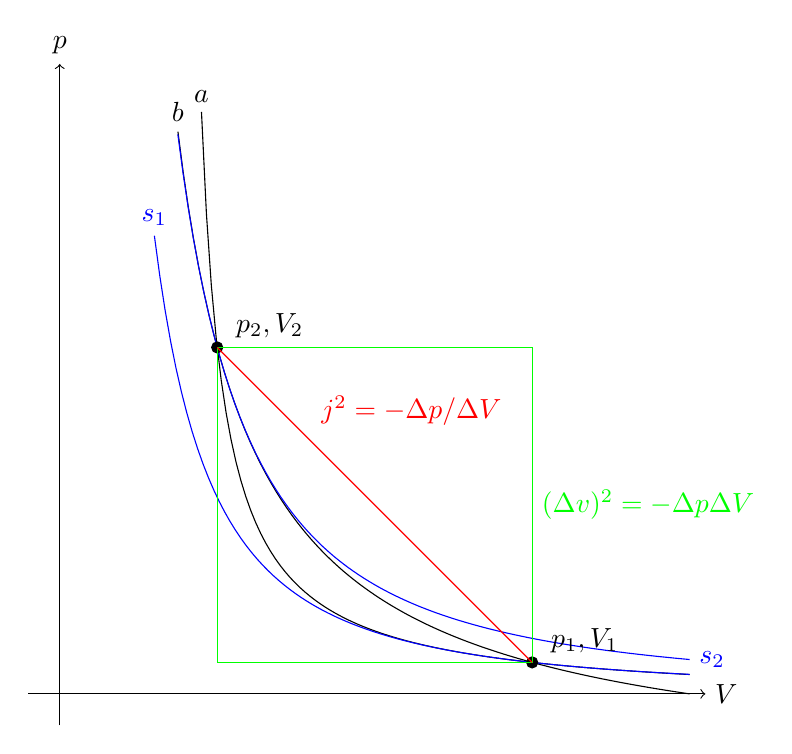
\begin{tikzpicture}
\begin{scope}[xscale=2,yscale=2]
\draw plot [domain=1.33333333:0.3,samples=100] ( 3*\x, { 0.2*(2.5 -
    0.5*(1+\x))/(2.5*\x-0.5*(1+\x))}) node [above] {$a$};
\draw plot [domain=1.33333333:0.25,samples=100] ( 3*\x, { 2.2*(5/6 -
  0.5*(1/3+\x))/(2.5*\x-0.5*(1/3+\x))}) node [above] {$b$};
\draw [blue] plot [domain=1.3333333:0.2,samples=100] ( 3*\x, {
  0.2*exp(-1.666667*ln(\x)) }) node [above] {$s_1$};
\draw [blue] plot [domain=0.25:1.3333333,samples=100] ( 3*\x, {
  2.2*exp(-1.666667*ln(3*\x)) }) node [right] {$s_2$};
\filldraw  (3,0.2) circle (1pt) node [above right] {$~p_1,V_1$}
           (1,2.2) circle (1pt) node [above right] {$~p_2,V_2$};
\draw [green] (3,0.2) rectangle (1,2.2) (3,1.2) node [right] { $(\Delta
  v)^2=-\Delta p \Delta V$};
\draw [red] (3,0.2) -- (1,2.2) (1.6,1.8) node [right] { $j^2 =
  -\Delta p/\Delta V$} ;
\draw [->] (-0.2,0)--(4.1,0) node [right] {$V$} ;
\draw [->] (0,-0.2)--(0,4) node [above] {$p$};
\end{scope}
\end{tikzpicture}
\end{center}
\caption{Shock (Hugoniot) Adiabats (in black) and Standard (Poisson)
  Adiabats (in blue)}
\label{fig:Hugoniot}
\end{figure}
\index{shocks!shock abiabat}
\index{fluid mechanics!Hugoniot abiabat}
\index{Hugoniot abiabat}
Fig.~\ref{fig:Hugoniot} depicts the shock or Hugoniot adiabat for a
shock with a preshock pressure $p_1$ and specific volume $V_1$.  Any
point along the curve $a$ to the left of $(p_1,V_1)$ is a possible
postshock condition.  A particular postshock condition $(p_2,V_2)$ is
highlighted. The minimum flux passing through the shock is
given by the negative of the slope at $(p_1,V_1)$, and it increases as
the shock gets stronger.  The velocity difference vanishes for small
shocks and grows as the area of the box as the shock grows.  

The curve
$b$ to the left of $(p_2,V_2)$ shows the possible postshock conditions
if the preshock condition is $(p_2,V_2)$.  Notice that it also
intersects the curve $a$ at $(p_1,V_1)$.  There are two (or no) shock adiabats
that connect any two points in the $p-V-$plane.  One corresponds to
pressure and density increasing through the shock (curve $a$), and one
corresponds to pressure and density decreasing through the shock
(curve $b$).   Earlier it was stated that these quantities must
increase through the shock, but no reason was given.
Fig.~\ref{fig:Hugoniot} shows the curves of constant entropy
or standard (Poisson) adiabats on the $p-V-$plane corresponding to the
values of the entropy at $(p_1,V_1)$, $s_1$, and  at $(p_2,V_2)$,
$s_2$.   We know that if the pressure is higher at a particular
density or specific volume than the entropy is larger so $s_2>s_1$.
From the second law of thermodynamics we know that entropy cannot
decrease in an isolated system, so the initial state of the flow must
be $(p_1,V_1)$ and the final state is $(p_2,V_2)$.  Furthermore, we
can see that the curves of constant entropy not only pass through the
correponding plots in the plane (this is by design) but they are also
tangent to and have the same radius of curvature as the shock
adiabats.  This means that both the first and second derivatives
coincide for these two sets of curves and that the increase in entropy
is third order in the size of the shock.

Although the curve $b$ that travels from $(p_2,V_2)$ to $(p_1,V_1)$ is
an unphysical solution for a shock because entropy decreases along the
path, it does provide some great insights.  What is the velocity of
the flow on either side of the shock?  We have
\begin{equation}
v_1^2 = j^2 V_1^2 = -\frac{\Delta p}{\Delta V} V_1^2~\textrm{and}~
v_2^2 = -\frac{\Delta p}{\Delta V} V_2^2.
\label{eq:849}
\end{equation}
What is the sound speed on either side of the shock?  We have
\begin{equation}
c_{s,1}^2 = \left . \frac{\partial P}{\partial \rho} \right |_{s_1} =
-V_1^2 \left . \frac{\partial P}{\partial V} \right |_{s_1} = -V_1^2
\left . \frac{\partial P}{\partial V} \right
|_{a}~\textrm{and}~c_{s,2}^2 = -V_1^2
\left . \frac{\partial P}{\partial V} \right |_{b}
\label{eq:850}
\end{equation}
so the Mach numbers on each side of the shock are given by the ratio
of the slope of the secant to the slope of the tangent.  That is,
\begin{equation}
M_1^2 =\frac{\Delta p}{\Delta V} \Big / {\left . \frac{\partial
      P}{\partial V} \right |_{a}}~\textrm{and}~M_2^2 = {
  \frac{\Delta p}{\Delta V} } \Big / {\left . \frac{\partial P}{\partial V} \right |_{b}}.
\end{equation}
Because all of the adiabats are concave up in the $p-V-$plane, the
slope of the secant must be larger than that of the tangent at $(p_1,V_1)$, so
the flow enters the shock supersonically.  Conversely at $(p_2,V_2)$
the slope of the secant must be smaller than that of the tangent, so the
flow exits the shock subsonically.  As the shock decreases in
intensity, the figure demonstrates that both Mach numbers approach
unity.
 

\section{A Spherical Shock - The Sedov Solution}
\label{sec:spher-shock-sedov}
\index{Sedov solution}
\index{fluid mechanics!Sedov solution}
\index{fluid mechanics!spherical shock}

Let's imagine that we dump a really large amount of energy into a
small region.  The energy is initially carried by a small mass ($m$).
Initially, as long as 
\begin{equation}
m \gg \frac{4}{3} \pi r^3 \rho.
\label{eq:708}
\end{equation}
where the right-hand side is the mass swept up.
The ejecta will freely expand.  Let's imagine sometime later when the
mass of the ejecta is negligible but that the energy of the explosion
is still large compared to the enthapy of the swept-up material
\begin{equation}
E \gg \frac{4}{3} \pi r^3 \rho w.
\label{eq:709}
\end{equation}
This is equivalent to $p_2 \gg p_1$, so we have a strong shock, so
$\rho_2/\rho_1 = (\gamma+1)/(\gamma-1)$

In this situation, we only have four numbers of interest,
\begin{itemize}
\item $r$, the distance from the centre of the explosion
\item $t$, the time since the explosion and
\item $E$, the energy of the explosion.
\item $\rho_1$, the density of the undisturbed gas
\end{itemize}
By combining $E$, $t$ and $\rho$ we can find only one expression with
the dimension of length, so let us take the radius of the shock to be
\begin{equation}
R(t) =  R_0 \left ( \frac{E t^2}{\rho_1} \right )^{1/5}.
\label{eq:710}
\end{equation}
where $R_0$ is a dimensionless constant that we will determine from
the solution.  The velocity of the shock wave with respect to the
undisturbed gas is
\begin{equation}
v_s = -v_{1,s} = \dd{R}{t} = \frac{2R}{5t} = \frac{2}{5} R_0 E^{1/5}
\rho_1^{-1/5} t^{-3/5}
\label{eq:711}
\end{equation}
We would like to know the speed of the gas relative to the undisturbed
gas after the shock has passed,
\begin{equation}
v_{2,s} - v_{1,s}  = v_{2,u} - v_{1,u} = v_{2,u}
\label{eq:712}
\end{equation}
For a strong shock we have
\begin{equation}
v_{2,u} = \frac{\gamma-1}{\gamma+1} v_{1,s} - v_{1,s} =
\frac{2}{\gamma+1} v_s
\label{eq:713}
\end{equation}
and
\begin{equation}
\rho_2 = \rho_1 \frac{\gamma+1}{\gamma-1}~\rmmat{and}~P_2 =
\frac{2}{\gamma+1} \rho_1 u_1^2.
\label{eq:714}
\end{equation}
Behind the shock, the fluid is ideal so we can use the continuity,
Euler and energy equations
\begin{eqnarray}
\pp{v}{t} + v \pp{v}{r} +\frac{1}{\rho} \pp{p}{r} &=& 0 \\
\pp{\rho}{t} +  \pp{(\rho v)}{r} + \frac{2\rho v}{r} &=& 0 \\
\left ( \pp{}{t} + v \pp{}{r} \right ) 
\ln \left (\frac{p}{\rho^\gamma} \right ) &=& 0.
\label{eq:715}
\end{eqnarray}
The final equation says that the entropy per unit mass does not
change.
The trick to solve these equations is to assume that all of the
variables depend on the similarity variable $\xi = [ r/R(t) ]$ with
the right scaling.  For example we have
\begin{equation}
v = \frac{2r}{5t} V(\xi), \rho = \rho_1 G(\xi), c_s^2 = \gamma
\frac{P}{\rho} = \frac{4 r^2}{25 t^2} Z(\xi).
\label{eq:716}
\end{equation}
The shock jump conditions give the boundary conditions for the
solution,
\begin{equation}
V(1) = \frac{2}{\gamma+1}, G(1) = \frac{\gamma+1}{\gamma-1}, Z(1) =
\frac{2\gamma (\gamma-1)}{(\gamma+1)^2}.
\label{eq:717}
\end{equation}

Padmanabhan gives a general solution to these equations in closed
form, but let's look at the results for $\gamma=5/3$ depicted in
Fig.~\ref{fig:sedov}.   In general the value of $V$ ranges between $1/\gamma$ at
$\xi=0$ and $2/(\gamma+1)$ at $\xi=1$; it doesn't change much
with the similarity variable; most of the change in the velocity from
the center to the edge comes from the scaling in Eq.~\ref{eq:716}
and the values of $G(\xi)$ and $Z(\xi)$ can be written in terms of
$V(\xi)$.   We can find one of these relationships by examining the
conservation of energy in the flow.  The total energy of the flow is
simply $E$ because no energy leaves the flow and the material swept up
by the shock is assumed to have no energy.  Furthermore, the flow is
self-similar so the energy contained within a spherical shell labelled
by the similarity variable $\xi$ must be constant with time.  Let's
look at a the flow at particular value of $\xi$.  The total energy
flowing outward through a spherical surface over a time $dt$ is 
\begin{equation}
d E = 4\pi r^2 \left ( w+\frac{v^2}{2}\right ) \rho v dt.
\end{equation}
On the other hand the volume swept out
as the flow expands self-similarly is 
\begin{equation}
d V = 4 \pi r^2 \left .\frac{\partial r}{\partial t}\right |_\xi d t.
\end{equation}
We can combine this with the energy density to yield the energy in the region
\begin{equation} 
d E = 4 \pi r^2 \left .\frac{\partial r}{\partial t}\right |_\xi
\left ( \epsilon + \frac{v^2}{2} \right ) \rho d t.
\end{equation}
We can equate these two energies and solve for $c_s^2 = \gamma P/\rho$ to give
\begin{equation}
Z(\xi) = \frac{\gamma(\gamma-1) V(\xi)^2 \left [ 1-V(\xi) \right ]}{2
  \left [ \gamma V(\xi) -1 \right ]}
\end{equation}

The final step in completing the solution is to find the relationship
between the energy of the explosion and the value of $R_0$. We have
\begin{equation}
E = \int_0^R 4 \pi r^2 dr \rho \left [ \frac{v^2}{2} + \epsilon \right
] =\int_0^R 4 \pi r^2 dr \rho \left [ \frac{v^2}{2} +
  \frac{c_s^2}{\gamma(\gamma-1)} \right ]
\end{equation}
and change variables to $\xi$ with $r=R(t) \xi$ to yield
\begin{equation}
E = R(t)^5 \rho_1 \frac{16\pi}{25 t^2} \int_0^1 \xi^4 G(\xi) \left [
  \frac{V(\xi)^2}{2} + \frac{ Z(\xi) }{\gamma(\gamma-1)} \right ] 
\end{equation}
and
\begin{equation}
1 = R_0^5 \frac{16\pi}{25} \int_0^1 \xi^4 G(\xi) \left [
  \frac{V(\xi)^2}{2} + \frac{ Z(\xi) }{\gamma(\gamma-1)} \right ],
\end{equation}
showing explicitly that the value of $R_0$ is a dimensionless number
that only depends on the value of $\gamma$.  The value $R_0$ is
approximately 1.033 for $\gamma=7/5$ and 1.152 for $\gamma=5/3$.  It
ranges from 0.783 to 1.232 as $\gamma$ goes from 1.1 to 1.9.
Amazingly without knowing $\gamma$ well one can get an estimate of the
energy of the blast (within a factor of three) simply from measuring
the value of the radius of the shock at a particular time and taking
$R_0=1$.
\begin{figure}
\begin{center}
\begin{tikzpicture}
\begin{scope}[xscale=5,yscale=3]
\draw plot file{sedov/sedovv.dat} ;
\draw (0.8,0.9) node {$v/v_2$} (0.1,0.4) node {$p/p_2$} (0.3,0.1) node
{$\rho/\rho_2$};
\draw plot file{sedov/sedovrho.dat} ;
\draw plot file{sedov/sedovp.dat} ; 
\draw [->] (-0.2,0)--(1.1,0) node [right] {$r/R$} ;
\draw [->] (0,-0.2)--(0,1.1) ;
\end{scope}
\end{tikzpicture}
\end{center}
\caption{Variation of the density, velocity and pressure behind the
  shock for the Sedov-Taylor blast wave}
\label{fig:sedov}
\end{figure}
% {
% \begin{figure}
% \centering
% \includegraphics[width=\textwidth]{sedov} 
% \caption{Sedov Solution}
% \label{fig:sedov}
% \end{figure}
% }

\section{Detonation Waves}
\label{sec:detonation-waves}
\index{fluid mechanics!detonation waves}

In a detonation as the material passes through the shock energy is
released either through chemical changes or nuclear burning.  One
could have either a release of energy through the shock (like
combustion) or a consumption of energy (like ionization).   The jump
conditions are with the exception of the energy equation
\begin{equation}
\frac{1}{2} v_1^2 + w_1 = \frac{1}{2} v_2^2 + w_2
\label{eq:853}
\end{equation}
where $w_1$ and $w_2$ are now different functions of $p$ and $V$ to
reflect the different chemical or nuclear composition of the gas
before and after the reactions.  Fig.~\ref{fig:Detonation} depicts the
situation graphically.  The lower curve $a$ is the shock adiabat
without the chemical changes and $a'$ is the detonation abiabat which
uses the functional form of the enthalpy in the burnt gas.  We still
have the relationships between the flux, velocities and slopes and
areas on the $p-V-$plane, because these originated from the
conservation of momentum and mass not from the energy equation that
has changed.
\index{shocks!detonation abiabat}
\index{fluid mechanics!detonation abiabat}

The various points outline how the gas changes as it passes through
the shock and burns.  An example of the general case, the gas enters
the shock supersonically at $A$ and is compressed to point $B$ and
leaves the shock subsonically and at the same time or after the gas
burns and moves along the chord to point $E$.  Because the flux of the
flow is conserved through the transition, the state of the gas must
remain on the chord $AB$.  There is a minimum flux that can pass
through the detonation front, $j_\mathrm{min}$, and this flux also
corresponds to the minimum velocity jump through the front where the
final state is $O$ or the Jouguet point.  In the
case of a shock without a chemical change there is no minimum velocity
jump.  

\index{Jouguet point}
\index{shocks!Jouguet point}
\index{Chapman-Jouguet condition}
Although the minimal value of the flux appears to be a special case,
it is actually occurs in nature often.  A detonation that proceeds
from $A$ to $D$ and then to $O$ minimizes the entropy incease in the
front. Furthermore, for final states above $O$ along $a'$ the gas
leaves the front subsonically.  If the final state lies at $O$, the
gas leaves the detonation front right at the speed of sound in the
downstream flow.  This special situation often arises when the
combustion itself creates the shock.  Let's take a specific example of
a detonation front that starts near the closed end of a tube.  The
front must be followed by a rarefaction wave that travels up the tube
at the speed of sound through the postshock gas.  If the postshock gas
is traveling subsonically relatively to the shock then the rarefaction
wave will eventually catch up to the back of the shock reducing the
flux through the shock by reducing the postshock pressure and shock
velocity relative to the preshock gas until the minimum flux is
achieved.  At this point the postshock gas leaves the front at the
sound speed so the rarefaction wave no longer overtakes the shock and
the combined detonation front and rarefaction wave achieves a steady
state.  The detonation adiabat below the Jouguet point $O$ cannot be
reached if the combustion begins after the gas is compressed.  The
point $E$ for example has a lower entropy than point $C$ so the gas
cannot pass from $C$ to $E$ either immediately after the shock or
through a subsequent shock.

% $\beta P_1/\rho_1$ is the energy per unit mass released or
% removed as material passes through the shock.  In this case
% Eq.~\ref{eq:837} stands but Eq.~\ref{eq:842} becomes
% \begin{equation}
% \frac{P_2}{P_1} = \frac{\rho_2}{\rho_1} \left ( 1 - \beta
%   \frac{\gamma-1}{\gamma} \right ) + \frac{1}{2} M_1^2 \left
%   (\gamma-1\right ) \left( \frac{\rho_2}{\rho_1} -
%   \frac{\rho_1}{\rho_2} \right ).
% \label{eq:843}
% \end{equation}
% It is apparent that we still have two solutions but $\rho_2=\rho_1$ is
% not one of them.

\begin{figure}
\begin{center}
\begin{tikzpicture}
\begin{scope}[xscale=2,yscale=2]
\draw [gray] plot [domain=1.33333333:0.3,samples=100] ( 3*\x, { 0.2*(2.5 -
    0.5*(1+\x))/(2.5*\x-0.5*(1+\x))}) node [above] {$a$};
\draw plot [domain=1.33333333:0.345,samples=100] ( 3*\x, { 0.4*(2.5 -
    0.5*(1+\x))/(2.5*\x-0.5*(1+\x))}) node [above] {$a'$};
% \draw [blue] plot [domain=1.3333333:0.2,samples=100] ( 3*\x, {
%   0.2*exp(-1.666667*ln(\x)) }) node [above] {$s_1$};
% \draw [blue] plot [domain=1.3333333:0.2,samples=100] ( 3*\x, {
%   0.4*exp(-1.666667*ln(\x)) }) node [above] {$s_1'$};
% \draw [blue] plot [domain=0.25:1.3333333,samples=100] ( 3*\x, {
%   2.2*exp(-1.666667*ln(3*\x)) }) node [right] {$s_2$};
\draw [blue] plot [domain=0.8:4,samples=100] ( \x, {
  0.7075383629*exp(-1.666667*ln(\x/2.1383708395)) }) node [right] {$s_O$};
\filldraw  (3,0.2) circle (1pt) node [ below left] {$A$} 
           (1,2.2) circle (1pt) node [above right] {$B$}
           (1.315,1.885) circle (1pt) node [above right] {$C$}
           (2.73,0.47) circle (1pt) node [above right] {$E$}
           (3, 0.2) ++(149.5:2.12) circle (1pt) node [above right] {$D$}
           (3, 0.2) ++(149.5:1) circle (1pt) node [below] {$O$};
% \draw [green] (3,0.2) rectangle (1,2.2) (3,1.2) node [right] {
% $(\Delta v)^2=-\Delta p \Delta V$};
\draw [red,dashed] (3,0.2) -- (1,2.2) (1.6,1.8) node [right] { $j^2 =
  -\Delta p/\Delta V$} ;
\draw [red] (3,0.2) -- ++(149.5:2.12) (2,0.8) node [left] { $j_\mathrm{min}^2$ };
\draw [->] (-0.2,0)--(4.1,0) node [right] {$V$} ;
\draw [->] (0,-0.2)--(0,4) node [above] {$p$};
\end{scope}
\end{tikzpicture}
\end{center}
\caption{Shock (Hugoniot) Adiabat (in gray), Detonation Adiabat (in
  black) and Standard (Poisson) Adiabat (in blue)}
\label{fig:Detonation}
\end{figure}

\section{Radiative Shocks}
\label{sec:radiative-shocks}
\index{fluid mechanics!radiative shocks}
\index{shocks!radiative}

So far we have assumed that the energy in a fluid element is conserved
through the shock, that no energy leaves the flow or is radiated.  The
opposite extreme is that the shock heats the gas sufficiently that
radiative losses are important near the shock and the gas rapidly
cools.  In this case we must abandon the conservation of energy flux
through the shock (Eq.~\ref{eq:704}) and find another criterion to
understand how the gas changes through the shock.  Astrophysically the
rate that gas cools can depend very sensitively on the temperature of
the gas.  In particular gas above about $10^4$~K radiates much more
effectively than cooler gas.  Imagine if the gas before the shock was
just below the critical temperature at which cooling set in.  As it
passes through the shock, it goes above this temperature and then
rapidly begins to cool and rapidly returns to its initial
temperature.  The additional condition that we seek is that final
temperature equals the initial temperature.
\index{shocks!isothermal}
\index{fluid mechanics!isothermal shocks}
\begin{figure}
\begin{center}
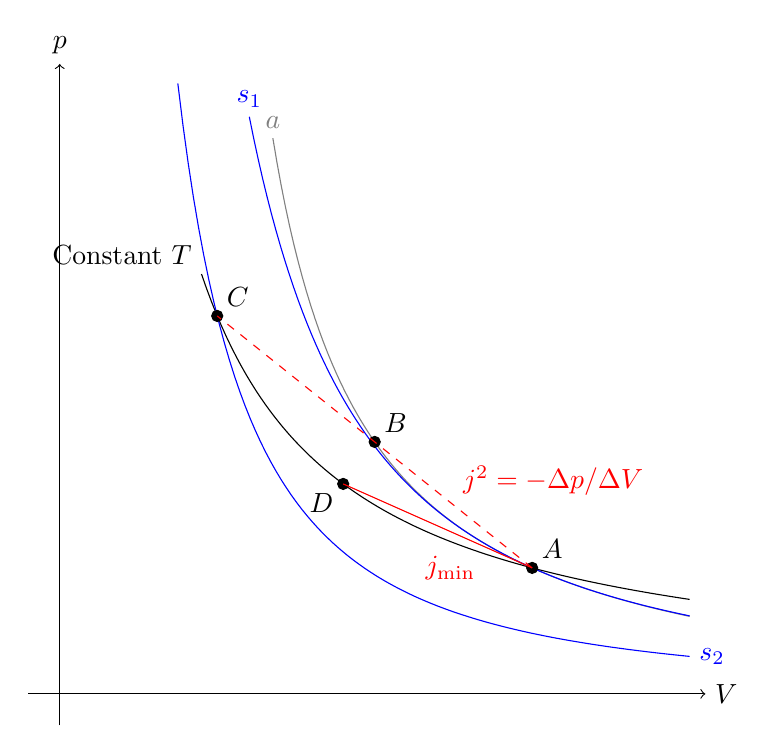
\begin{tikzpicture}
\begin{scope}[scale=2]
\draw [gray] plot [domain=1.33333333:0.45,samples=100] ( 3*\x, { 0.8*(2.5 -
    0.5*(1+\x))/(2.5*\x-0.5*(1+\x))}) node [above] {$a$};
\draw plot [domain=1.33333333:0.3,samples=100] ( 3*\x, { 0.8/\x}) node
[above left] {Constant $T$};
\draw [blue] plot [domain=1.3333333:0.4,samples=100] ( 3*\x, {
  0.8*exp(-1.666667*ln(\x)) }) node [above] {$s_1$};
\draw [blue] plot [domain=0.25:1.3333333,samples=100] ( 3*\x, {
  2.4*exp(-1.666667*ln(3*\x)) }) node [right] {$s_2$};
\filldraw  (3,0.8) circle (1pt) node [above right] {$A$}
           (2,1.6) circle (1pt) node [above right] {$B$}
           (1,2.4) circle (1pt) node [above right] {$C$}
           (1.8,1.3333333) circle (1pt) node [below left] {$D$};
\draw [dashed,red] (3,0.8) -- (1,2.4) node [pos=0.25, above right] { $j^2 =
  -\Delta p/\Delta V$} ;
\draw [red] (3,0.8) -- (1.8,1.3333333) node [pos=0.25, below left] {
  $j_\mathrm{min}$ } ;
\draw [->] (-0.2,0)--(4.1,0) node [right] {$V$} ;
\draw [->] (0,-0.2)--(0,4) node [above] {$p$};
\end{scope}
\end{tikzpicture}
\end{center}
\caption{Isotherm (in black), Shock (Hugoniot) Adiabat (in gray), Standard (Poisson)
  Adiabats (in blue)}
\label{fig:isothermalshock}
\end{figure}

Again we still have the relationships between the flux, velocities,
slopes and areas on the $p-V-$plane that result from the conservation
of momentum and mass, but the shock adiabat is replaced with an
isotherm as shown in Fig.~\ref{fig:isothermalshock}.  From the diagram
it is apparent that the entropy of the gas decreases through an
isothermal shock; as a gas is compressed at constant temperature, its
entropy decreases.  The radiation carries away both energy and
entropy.  Because the standard adiabats are generally steeper than the
isotherms, the gas always leaves the shock subsonically.  Again
because the momentum flux is conserved, the gas must remain on the
chord $AC$ throughout.   As it passed through the shock it is heated
from $A$ to point $B$ and then as it cools it travels from $B$ to $C$.
As for the case of a detonation, we find that there is a minimum flux
that can pass through an isothermal shock and a minimal velocity
change.  Just above the flux $j_\mathrm{min}$ the flow enters the
shock slightly supersonically and leaves subsonically.

The initial and final Mach numbers and densities are related through
\begin{equation}
M_2 = \frac{1}{\gamma M_1}, \frac{\rho_2}{\rho_1} = \gamma M_1^2, \frac{P_2}{P_1} = \gamma M_1^2.
\label{eq:678}
\end{equation}
The ratio of the energy flux entering the radiative shock to that
leaving is given by
\begin{equation}
\frac{q_1}{q_2} = \gamma^2 M_1^2 \frac{(\gamma-1) M_1^2 + 2}{2 \gamma^2
  M_1^2 + \gamma - 1}.
\end{equation}
For large values of $M_1$ the initial energy flux is much larger than
the final energy flux.  At the other end the minimum value of $M_1$ is
of course unity. This yields a minimum energy ratio for the isothermal
shock of
\begin{equation}
\left .  \frac{q_1}{q_2} \right |_\mathrm{min} = \frac{\gamma^2}{2
  \gamma -1}.
\end{equation}
Even this weakest of isothermal shocks results in a compression ratio
$\rho_2/\rho_1 = \gamma$.

Sometimes the temperature of the gas is held constant through the
interaction with an external radiation field, so that even slight
departures from isothermality disappear on a short timescale.  In this
case it makes sense to take $\gamma=1$.   If we substitute $\gamma=1$
in Eq.~\ref{eq:679} through~\ref{eq:706} we obtain Eq.~\ref{eq:678}.
However, the enthalpy of an isothermal gas is given by
\begin{equation}
  w = c_s^2 \ln \left ( \frac{\rho}{\rho_0} \right ),
\end{equation}
so if we take the reference density $\rho_0=\rho_1$ we find
\begin{equation}
\frac{q_1}{q_2} = \frac{M_1^4}{1+\ln M_1^4}
\label{eq:757}
\end{equation}

\section{Relativistic Shocks}
\label{sec:relativistic-shocks}
\index{fluid mechanics!relativistic shock waves}
\index{shocks!relativistic}

We will look at relativistic shocks as an example of relativistic
hydrodynamics.  In particular we will look at the relativistic jump
conditions across the shock.  The particle flux must be conserved
across the shock (Eq.~\ref{eq:616})
\begin{equation}
J_{x,1} = J_{x,2}, \frac{U_1}{V_1} = \frac{U_2}{V_2}
\label{eq:854}
\end{equation}
where $V_1=1/n_{\mathrm{prop},1}$ and $U_1 = \gamma_1 v_1/c$
is the spatial component of four-velocity of the flow before the shock
and $\gamma_1=(1-v_1^2/c^2)^{-1/2}$.  It is most clear to use the
rest-mass energy density for $n_\mathrm{prop}$.  The components of the
stress-energy tensor must also be conserved (Eq.~\ref{eq:627})
\begin{equation}
T_{x0,1}=T_{x0,2}, w_1 U_1 \gamma_1= w_2 U_2 \gamma_2
\label{eq:855}
\end{equation}
and
\begin{equation}
T_{xx,1}=T_{xx,2}, w_1 U_1^2 + p_1 = w_2 U_2^2 + p_2
\label{eq:856}
\end{equation}
where $w=\epsilon + p$ and $\epsilon$ includes the rest-mass energy of
the particles.  Here $w$ is the enthalpy per unit volume whereas in
previous sections it denoted the enthalpy per unit mass,
$w_\mathrm{mass}=w_\mathrm{volume} V$.

By combining the particle flux, Eq.\ref{eq:854}, and the momentum
equations, Eq.~\ref{eq:856}, we obtain the results
\begin{eqnarray}
j^2 &=& \frac{p_2-p_1}{w_1 V_1^2 - w_2 V_2^2} = \frac{p_2-p_1}{V_{w,1} - V_{w,2}}, 
\label{eq:859}
\\
\left( U_1 - U_2 \right )^2 &=&
j^2 \left( V_1 - V_2 \right )^2  =  \frac{V_1-V_2} {V_{w,1}-V_{w,2}}
\left (p_2 - p_1 \right ) \left ( V_1 - V_2 \right )
\label{eq:857}
\end{eqnarray}
where $V_w = w V^2=(p + \epsilon ) V^2$.  These are analogous to
Eq.~\ref{eq:845} and~\ref{eq:848}.  Finally we can derive the equation
of the shock adiabat, using the identity $\gamma^2 = 1 + U^2$, to
yield
\begin{equation}
  w_1 V_{w,1} - w_2 V_{w.2} + \left( V_{w,1} + V_{w,2} \right ) \left (p_2 - p_1 \right ) = 0
\label{eq:860}
\end{equation}
which is very close in form to Eq.~\ref{eq:847}.  In the
non-relativistic limit for the second term we can take $V_w=V$,
but we must look at the first terms more closely because the result
depends on the difference of two quantities that are equal to lowest
order in the non-relativistic limit.  In particular,
\begin{equation}
w_1 V_{w,1} = w_1^2 V_1^2 = \left ( \rho_1 c^2 + w_{NR,1} \right )^2
V_1^2 = 1 + 2 w_{NR,1} V_1 + w_{NR,1}^2 V_1^2
\label{eq:861}
\end{equation}
where we have used $\rho_1 c^2 V_1=1$.  We can drop the last term.
The first term cancels in Eq.~\ref{eq:860}, leaving the middle term
which equals twice the enthalpy per unit mass and results in
twice Eq.~\ref{eq:847}.

\section{Hydraulic Jump}
\label{sec:hydraulic-jump}
\index{fluid mechanics!hydraulic jump}
\index{shocks!hydraulic jump}
Let's revist the dynamics of water travelling down a shallow channel.
We neglect the vertical motion of the fluid and assume that all
dimensions are large compared with the depth of the fluid --- this is the
{\em hydraulic} approximation.  If the flow only depends on the
position $x$ along the channel and time $t$, the continuity and
momentum equation are
\begin{equation}
\pp{h}{t} + \pp{(vh)}{x} = 0, \pp{v}{t} + v \pp{v}{x} = -g \pp{h}{x}.
\label{eq:862}
\end{equation}
where the depth $h$ is assumed to be constant across the channel.  We
can define a surface density ${\bar \rho} = \rho h$ and a mean
pressure ${\bar p}=\rho g h^2/2$ and recast the equations as
\begin{equation}
\pp{\bar \rho}{t} + \pp{(v {\bar \rho}}{x} = 0, \pp{v}{t} + v \pp{v}{x} =
-\frac{1}{\bar \rho} \pp{\bar p}{x}.
\label{eq:862}
\end{equation}
These equations are identical to the equations for the adiabatic flow
of a gas with $\bar p \propto \bar \rho^2$.  We can apply the results
from gas dynamics to hydraulics as along as the flow is abiabatic ---
no shocks.

These equations do not include the conservation of energy equation
because we assume that the flow does not have any internal energy or
entropy.  In practice the energy in the flow can be transferred to
small scale motion of the fluid which is quickly dissipated.  Let us
examine discontinuities in the fluid height and velocity by using the
conditions of continuity on the particle and momentum flux.  Such
discontinuities are known as {\em hydraulic jumps}. The mass
flux density is simply $j=\rho v h$ and the momentum flux is
\begin{equation}
\int_0^h \left ( p + \rho v^2 \right ) dz = \frac{1}{2} \rho g h^2 +
\rho v^2 h.
\label{eq:863}
\end{equation}
The jump conditions are 
\begin{equation}
v_1 h_1 = v_2 h_2, v_1^2 h_1 + \frac{1}{2} g h_1^2= v_2^2 h_2 + \frac{1}{2} g h_2^2.
\label{eq:864}
\end{equation}
We can express any two quantities in terms of the others in particular
we have the velocities in terms of the heights
\begin{equation}
v_1^2 = \frac{1}{2} g \frac{h_2}{h_1} \left ( h_1 + h_2 \right ),
v_2^2 = \frac{1}{2} g \frac{h_1}{h_2} \left ( h_1 + h_2 \right ).
\label{eq:865}
\end{equation}
If we look at the energy flux in the channel we have
\begin{equation}
q = \int_0^h \left ( \frac{p}{\rho} + \frac{1}{2}v^2 \right ) \rho v
dz = \frac{1}{2} j \left ( g h + v^2 \right ) 
\label{eq:866}
\end{equation}
and the difference in energy flux is
\begin{equation}
q_1 - q_2 = g j \frac{\left (h_1^2 + h_2^2 \right ) (h_2 - h_1)}{4 h_1
  h_2}. 
\label{eq:867}
\end{equation}
Because the energy flux of the flow must decrease through the jump
$h_2>h_1$ --- the height of the fluid must increase downstream of the
jump.  Substituting $h_2<h_1$ into Eq.~\ref{eq:865} shows that $v_1 .
\sqrt{g h_1}$ and $v_2 > \sqrt{g h_2}$.  The flow enters the jump
supercritically and leaves the jump subcritically.

\section{Problems}
\begin{enumerate}

\item{\bf Shock Entropy}
  Show that the entropy of the fluid increases as it passes
  through a shock. Hint: the equation of state of an isentropic fluid
  is $P = K\rho^\gamma$ where the value of $K$ increases with
  increasing entropy.

\begin{figure}
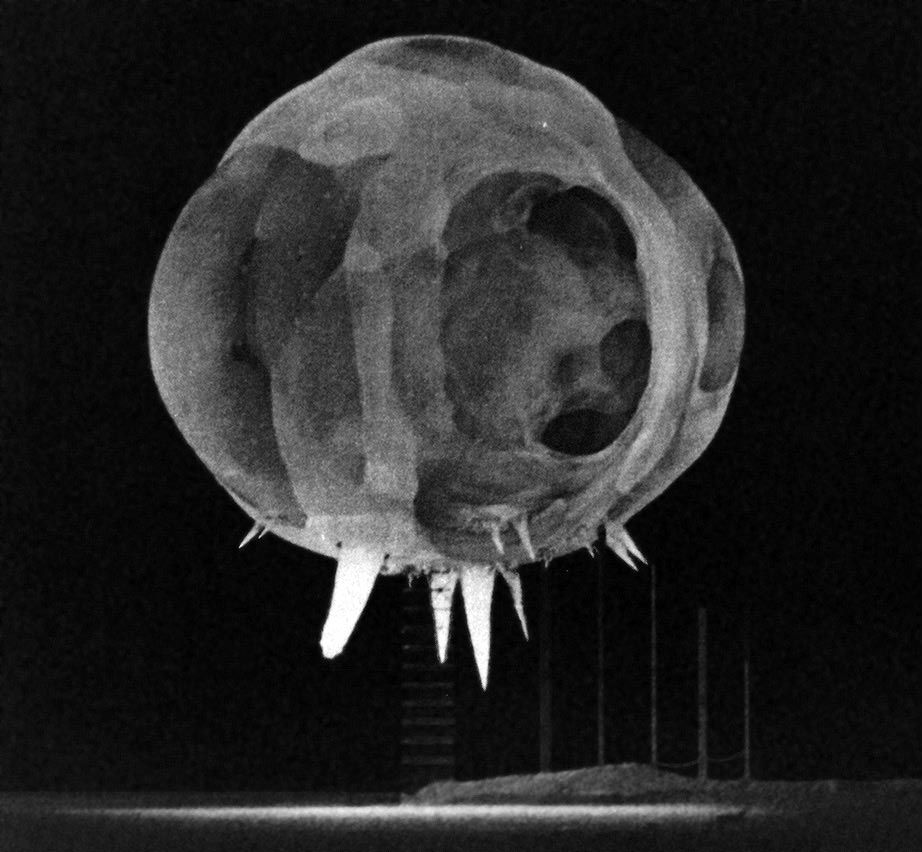
\includegraphics[width=\textwidth]{Tumbler_Snapper_rope_tricks.jpg}  
\caption{The explosion of nuclear device in 1952 about 2~ms after detonation.}
\label{fig:tumbler}
\end{figure}

\item{\bf Bomb Yield}

  Fig.~\ref{fig:tumbler} shows shocked air heated to incandescence
  about two milliseconds after the detonation of a nuclear
  bomb.  The height of the device was 90~meters.  What
  was the approximate yield of the device?

\item{\bf Relativistic Shock}

  Find the incoming and outgoing velocity of a relativistic shock in
  terms of the energy density and pressure on either side of the
  shock.

\item{\bf Relativistic Bernoulli}

  Find the relativistic generalisation of Bernoulli's equation for a
  streamline (you can neglect gravitiy).

\item{\bf Bathtub Physics}

  When water flows into a bathtub, a circular hydraulic jump forms
  around the incoming stream of water.  If you assume that the flow
  rate is constant and the flow is initially vertical, calculate the
  height of the water downstream of the jump as a function of the
  radius of the jump and the flow rate.  You may neglect friction and
  assume that the velocity upstream of the jump is constant. If
  the bathtub is large compared to the radius of the jump and the
  walls are vertical, how does the radius of the jump change with
  time?
\end{enumerate}
%%% Local Variables:
%%% TeX-master: "book"
%%% End:
